\section{Subject Area}

\begin{frame}
   \frametitle{\secname\ Overview}
   \tableofcontents[currentsection]
\end{frame}

\subsection{Clique}
\begin{frame}{\subsecname}
   A graph clique is a subset of its nodes such that it is fully connected.

   We will work mainly with 3-cliques, and often will refer to them as triangles.

   \begin{figure}[H]
       \centering
       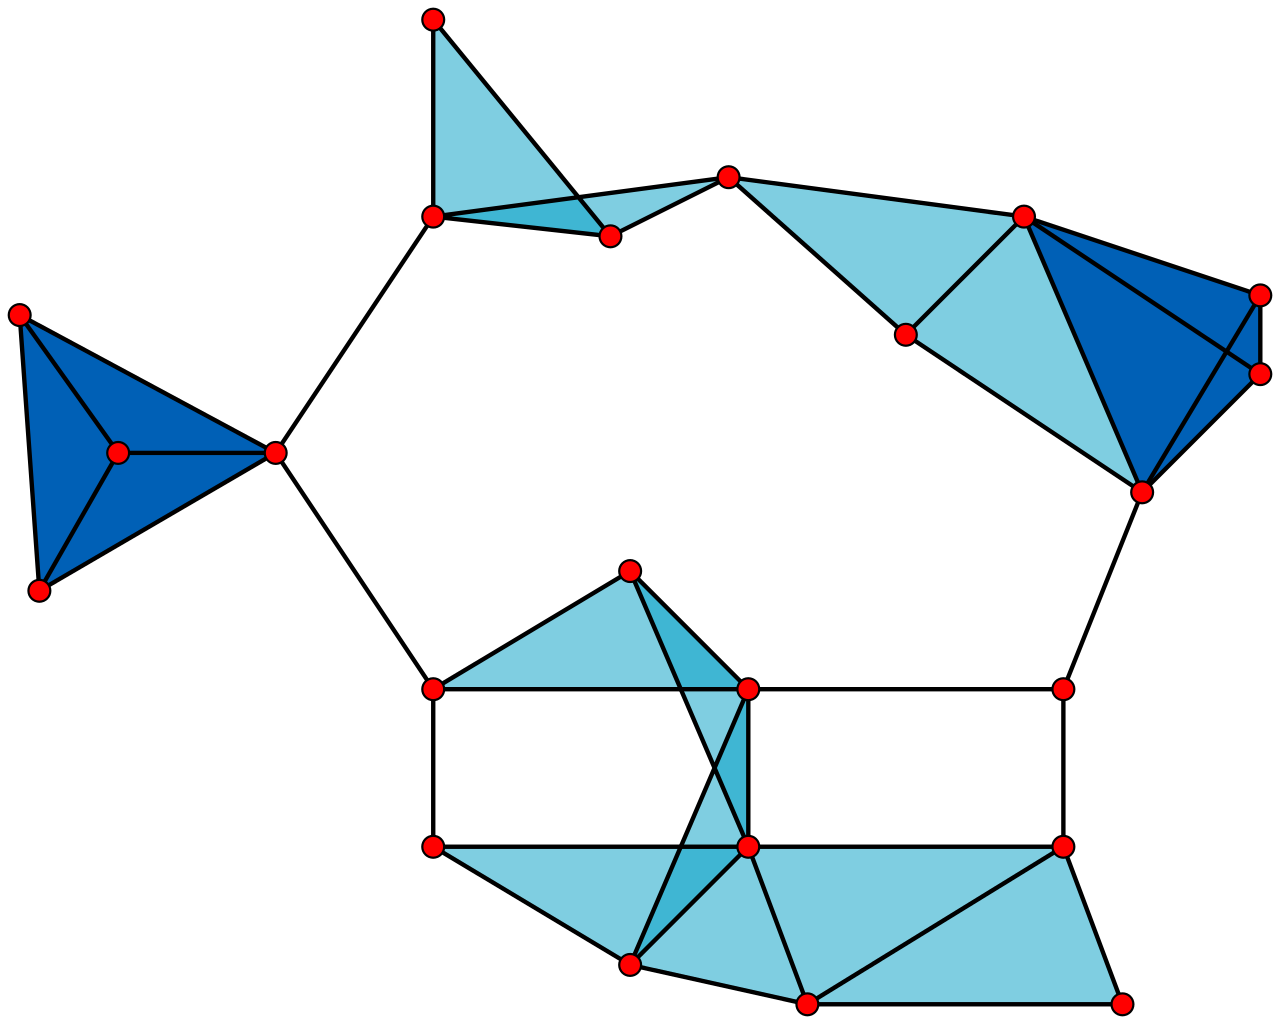
\includegraphics[height=0.6\textheight]{clique.png}
   \end{figure}
\end{frame}

\subsection{Incidence Matrix}
\begin{frame}{\subsecname}
   If we have an undirected graph $(V, E)$, its incidence matrix $\nabla$ of size $\lvert V \rvert \times \lvert E \rvert$ such that $A_{i, j} = 1$ if $i$-th vertex is a vertex of $j$-th edge.
   It shows relations between nodes and edges.

   \begin{multicols}{2}
       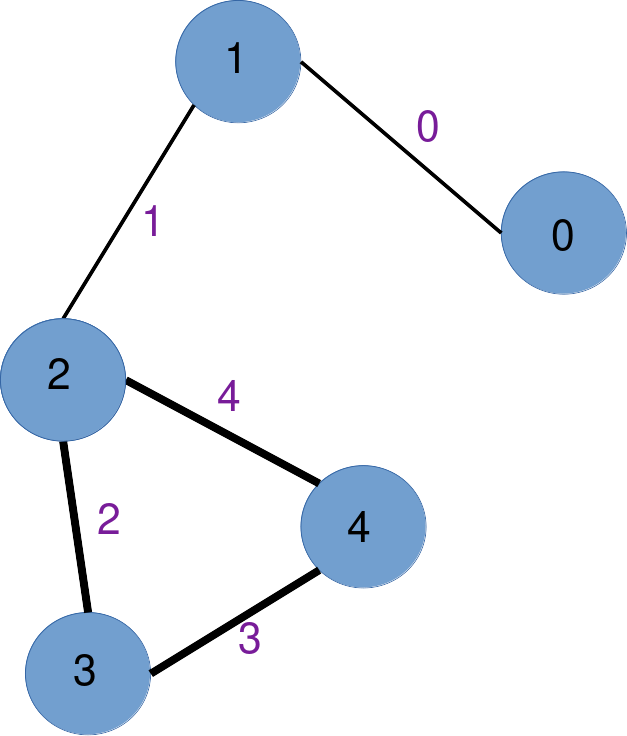
\includegraphics[width=0.3\textwidth]{incidence.png}

       \[
           \begin{bmatrix}
               1 & 0 & 0 & 0 & 0 \\
               1 & 1 & 0 & 0 & 0 \\
               0 & 1 & 1 & 0 & 1 \\
               0 & 0 & 1 & 1 & 0 \\
               0 & 0 & 0 & 1 & 1 \\
           \end{bmatrix}
       \]

   \end{multicols}
\end{frame}

\subsection{Laplacian matrix}
\begin{frame}{\subsecname}
   Another matrix representation of a graph.
   Usually is calculated using the following formula:
   \begin{equation*}
       L_{i, j} =
       \begin{cases}
           \deg(v_i) & \mbox{if}\ i = j                                                 \\
           -1        & \mbox{if}\ i \neq j\ \mbox{and}\ v_i \mbox{ is adjacent to } v_j \\
           0         & \mbox{otherwise},
       \end{cases}
   \end{equation*}

   However, other definitions also take place: $L = D - A$, where $D$ is a degree matrix and $A$ is an adjacency matrix.
   Another way to calculate a Laplacian is $L = \nabla\nabla^{T}$, where $\nabla$ is an incidence matrix.
\end{frame}

\subsection{Convolutional Graph Network}
\begin{frame}[allowframebreaks]{\subsecname}
   A type of GNN which generalizes the convolution operation to graphs.

   \begin{multicols}{2}
      \centering
      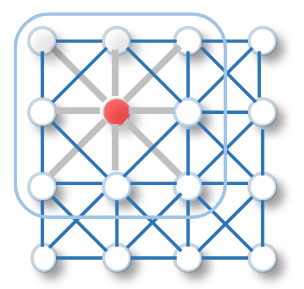
\includegraphics[width=0.4\textwidth]{conv.png}
      \caption{Convolution on image}
      \hfill
      \centering
      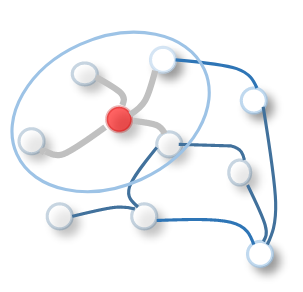
\includegraphics[width=0.4\textwidth]{CGN_conv.png}
      \caption{Convolution on graph}
   \end{multicols}
   
   \framebreak

   Assume we have a graph of $N$ nodes, where each node has $F$ features.
   We can construct an $N \times F$ matrix called feature matrix.
   The first layer takes the feature matrix, and performs the following operation: $Z = D^{-\frac{1}{2}} A D^{-\frac{1}{2}} X W$, where:
   \begin{itemize}
       \item $Z$ is resulting $N \times C$ signal
       \item $D$ is $N \times N$ degree matrix
       \item $A$ is $N \times N$ adjacency matrix with self-loops
       \item $X$ is $N \times F$ feature matrix (input signal)
       \item $W$ is $F \times C$ learnable weight matrix
   \end{itemize}

   The last (output) layer usually applies \emph{softmax} function to each row resulting in a new matrix $S$.
   Then, in order to classify a node $v_i$ we simply take the index of maximum of $S_i$.
   
   \framebreak

   The architecture of a graph convolutional network is presented on the figure below.
   \begin{figure}[h]
       \centering
       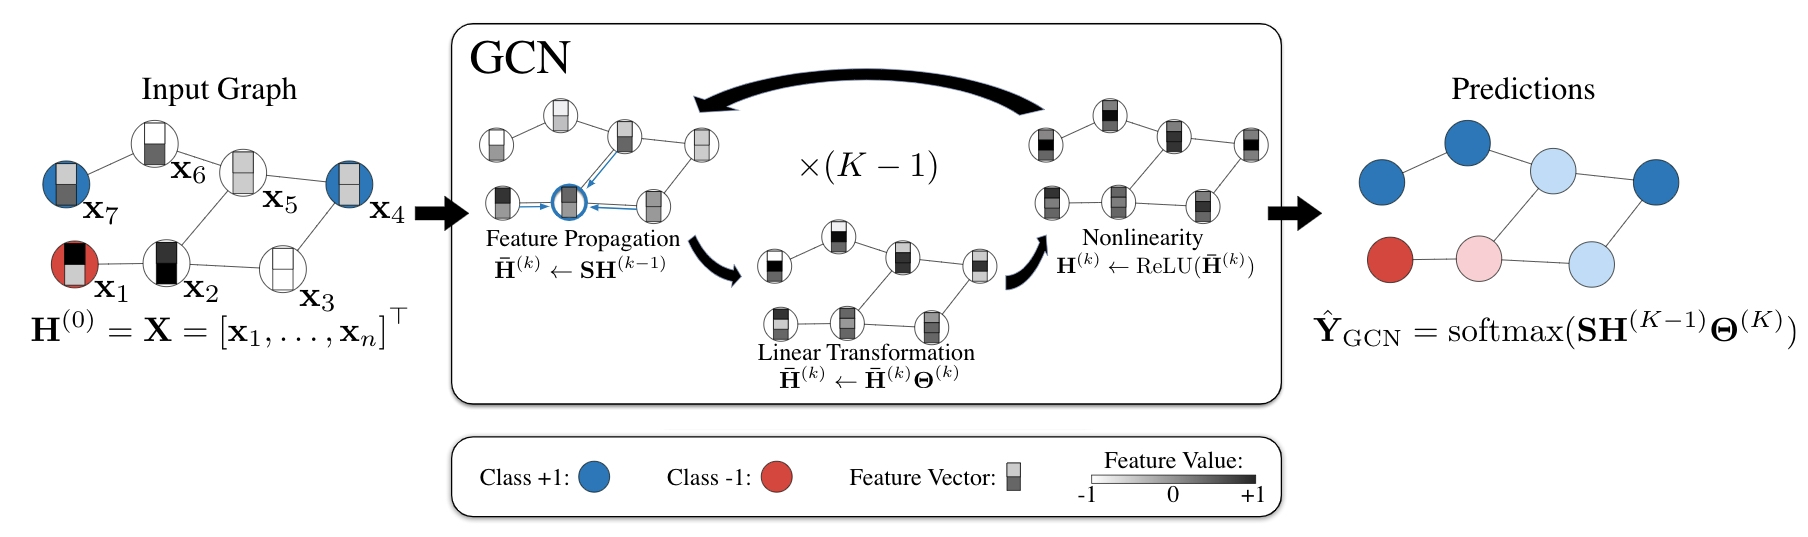
\includegraphics[width=\textwidth]{gcn.jpg}
   \end{figure}
\end{frame}

\subsection{Graph Attention Network}
\begin{frame}[allowframebreaks]{\subsecname}
   A type of GNN which uses attention mechanism (also borrowed from `casual' neural networks) which allows us to work with inputs of variable sizes and to focus on the most important features.
   The attention mechanism is a function $a: \mathbb{R}^C \times \mathbb{R}^C \rightarrow \mathbb{R}$ which takes two feature vectors $X_i, X_j$ and returns a scalar representing how tight the connection between $v_i$ and $v_j$ is.
   
   \framebreak

   We introduce an $N \times N$ matrix $e$ storing the attention between the nodes: $e_{i, j} = a\left( W \cdot X_i,\ W \cdot X_j \right)$.

   \textbf{Don't calculate all pairwise attentions!}
   One suggested solution is to use a neighborhood $\mathcal{N}_i$ of a vertex $v_i$ and then compute the attentions between $v_i$ and its' neighbors.
   Existing models uses neighborhood of size 1, and perform great.

   One might also want to normalize the coefficients.
   In order to do that, we can apply \empf{softmax} function: $c_{i, j} = \text{softmax}_j \left( e_{i, j} \right)$.

   \begin{figure}[h]
       \centering
       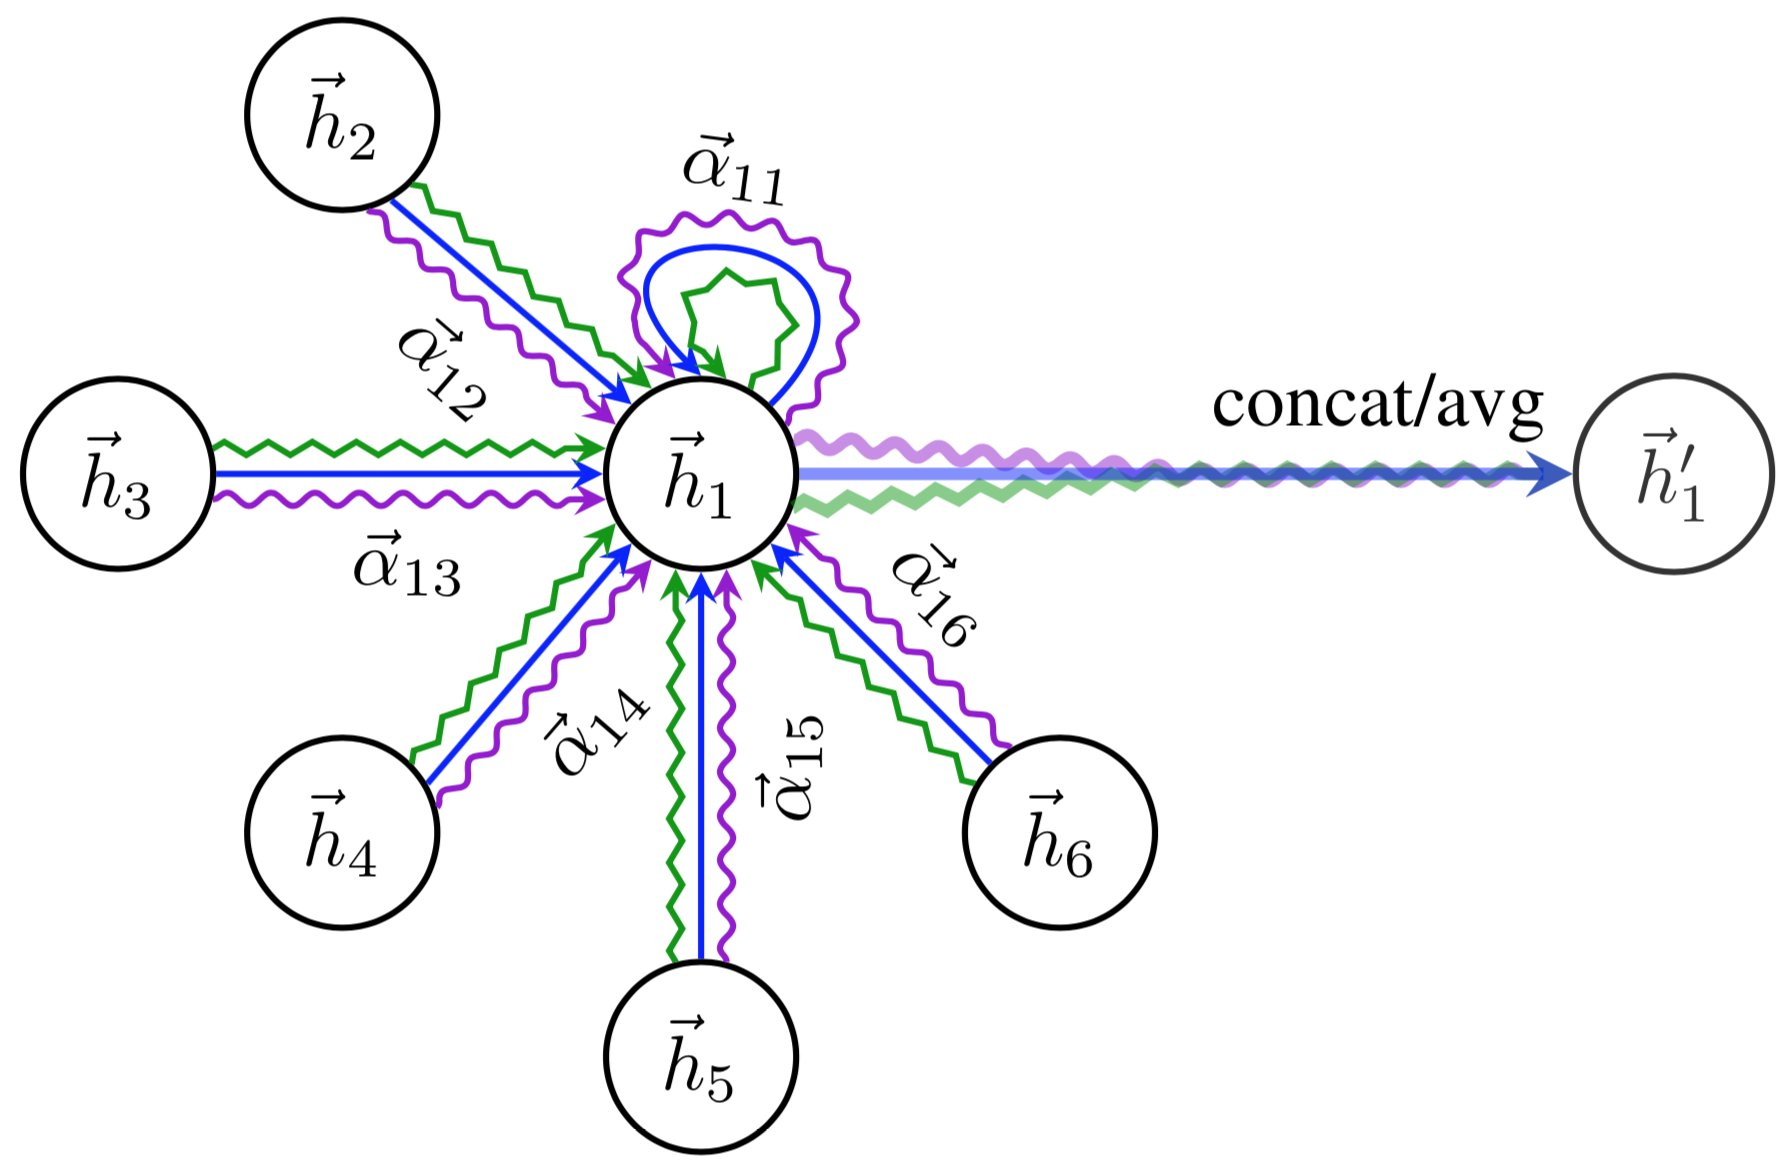
\includegraphics[width=0.7\textwidth]{gat.jpeg}
       \caption{An example of multi-head attention in a neighborhood of size 1}
   \end{figure}
\end{frame}

\subsection{Tasks solved by GNNs}
\begin{frame}{\subsecname}
   \begin{itemize}
      \item Node classification
      \item Graph classification
      \item Link prediction
   \end{itemize}
\end{frame}

\subsection{Relevance}
\begin{frame}{\subsecname}
   \begin{itemize}
      \item The field is new, therefore, there is a lot of space for improvement
      \item GNNs allow us to analyze complex relations with great precision
      \item We can improve the performance by preprocessing the data
      \item We can improve models by tweaking them
   \end{itemize}
\end{frame}
